\documentclass[12pt, a4papre]{article}
\usepackage[catalan]{babel}
\usepackage[unicode]{hyperref}
\usepackage{amsmath}
\usepackage{amssymb}
\usepackage{amsthm}
\usepackage{xifthen}
\usepackage{siunitx}
\usepackage{xcolor}
\usepackage{float}
\usepackage[utf8]{inputenc}

\usepackage{listings}
\usepackage{setspace}
\usepackage{graphicx}
\usepackage{tikz,lipsum,lmodern}
\usepackage[most]{tcolorbox}
\usepackage{circuitikz}
\usepackage{indentfirst}
\usepackage{verbatimbox}
\definecolor{mygreen}{RGB}{28,172,0} % color values Red, Green, Blue
\definecolor{mylilas}{RGB}{170,55,241}
\usepackage{listings}
\lstdefinelanguage{vhdl}{
   morekeywords={
     library,use,all,entity,is,port,in,out,end,architecture,of,
     begin,and
   },
   morecomment=[l]--
}
\usepackage{xcolor}
\colorlet{keyword}{blue!100!black!80}
\colorlet{comment}{green!50!black!90}
\lstdefinestyle{vhdl}{
   language     = VHDL,
   basicstyle   = \ttfamily,
   keywordstyle = \color{keyword}\bfseries,
   commentstyle = \color{comment}
}

\graphicspath{ {./Imatges/} }


\newcommand{\norm}[1]{\lvert #1 \rvert}

\hypersetup{
    colorlinks = true,
    linkcolor = blue
}

\author{Daniel Vilardell\\
	   Igor Yuziv}
\title{Memoria Practica 2}
\date{}

\begin{document}
	\maketitle
	\tableofcontents
     
     \newpage

	\section{Diseny Jerarquic}
	
	El diseny te l'objectiu de multiplicar dos nombres compresos entre 0 i 9 entrats desde la graella de la placa. Nomes es podra entrar dades quan el estat intro estigui activat i nomes es veurà el resultat quan estiguem en el estat show. El estat intro s'activa clicant al boto asterisc mentres que el estat show s'activa si es clica el botó coixinet. 
	
	El diseny principal \textbf{ppal} el que fa es rebre la tecla premuda i el bloc keygroup ens diu si es un coixinet, un asterisc o un nombre. Control rebra aquesta informacio i decidirà si mostra o no el resultat en funcio del estat que esta. També decidirà si deixa entrar dades o no, i en el cas que si, la sortida intro sera 1 i el bloc regs actualitzara el nombre amb el rebut per la tecla. Finalment els valors de opA i opB guardats es multipliquen i si estem en el estat de show es mostra el resultat, i si no no es mostra.
	
	El diseny exterior, que te la finalitat de comunicar el programa principal amb la placa desde la que introduim les dades funciona de la seguent manera.
	
	FALTA ACABAR LA EXPLICACIÓ
	
	\section{Blocs}
	
	\subsection{Conversor binari a BCD de 8 bits}
	
	Aquest component el farem amb vhdl i te l'objectiu de convertir la sortida del multiplicador de 8 bits a bcd per tal de mostrar a la placa. Te la seguent forma
	\begin{lstlisting}[style=vhdl, frame=single, basicstyle=\tiny]
LIBRARY ieee; USE ieee.std_logic_1164.ALL;  

ENTITY BIN_BCD_8B IS PORT (   
	BIN : IN STD_LOGIC_VECTOR(7 downto 0);   
	BCD : OUT STD_LOGIC_VECTOR(7 downto 0)); 
END BIN_BCD_8B;  

ARCHITECTURE taula_veritat OF BIN_BCD_8B IS   
	BEGIN 
	with BIN SELECT BCD <=     	
		"10011001" WHEN "00111000",  -- 81     
		"01110010" WHEN "01001000",  -- 72      
		"01100100" WHEN "01000000",  -- 64     
		"01010110" WHEN "00111000",  -- 56     
		"01010100" WHEN "00111000",  -- 54        
		"01001001" WHEN "00110001",  -- 49     
		"01001000" WHEN "00110000",  -- 48     
		"01000101" WHEN "00101101",  -- 45     
				.
				.
				. 
		"--------" WHEN OTHERS;   
END taula_veritat;


\end{lstlisting}

	\begin{table}[h!]
		\centering
		 \begin{tabular}{|c | c|} 
			 \hline
			 Entrades & Descripció\\ [0.5ex] 
			 \hline
			 BIN(8) &  Nombre en binari que es vol convertir a BCD\\ 
			 \hline\hline
			 Sortides & Descripció\\ [0.5ex] 
			 \hline
			 BCD(8) & Nombre BIN convertit a BCD\\ 
			 \hline
		 \end{tabular}
	\end{table}
	
	FALTA SIMULACIO
	
	Podem veure que la simulacio funciona ja que la entrada en binari es igual que la sortida en hexadecimal, es a dir, en BCD.
	
	\subsection{Conversor de binari de 4 bits a 8 bits}
	
	Aquest component el conectarem abans de la entrada del multiplicador per a transformar la entrada de 4 bits a la que necessita el multiplicador que es de 8 bits. Aquest l'unic que farà es omplir de 0 les primeres 4 entrades.
	\begin{figure}[H]
		\begin{center}
		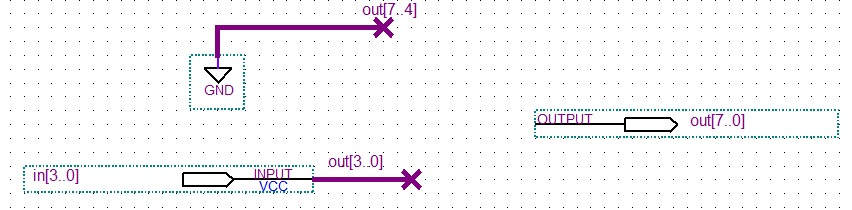
\includegraphics[width=130mm]{Bin_4_8.jpeg}
		\end{center}
	\end{figure}
	
	\begin{table}[h!]
		\centering
		 \begin{tabular}{|c | c|} 
			 \hline
			 Entrades & Descripció\\ [0.5ex] 
			 \hline
			 in(4) &  Nombre de 4 bits\\ 
			 \hline\hline
			 Sortides & Descripció\\ [0.5ex] 
			 \hline
			 out(8) & Sortida de 8 bits\\ 
			 \hline
		 \end{tabular}
	\end{table}
	
	FALTA SIMULACIÓ
	
	Podem veure que el component funciona a partir de la simulació ja que els nombres son els mateixos que els de la sortida pero la sortida te 8 bits en contes de 4.
	
	\subsection{Multiplicador}
	
	Aquest component t'he l'objectiu de multiplicar 2 nombres de 4 bits i treure la sortida en BCD de 4 bits, es a dir, 8 bits de sortida. Per a fer això usarem el component creat a la practica anterior que et multiplicava dos nombres de 8 bits. A la entrada hi posarem un conversor de 4 a 8 bits i a la sortida un conversor de binari de 8 bits a BCD que crearem amb vhdl.
	
	\begin{figure}[H]
		\begin{center}
		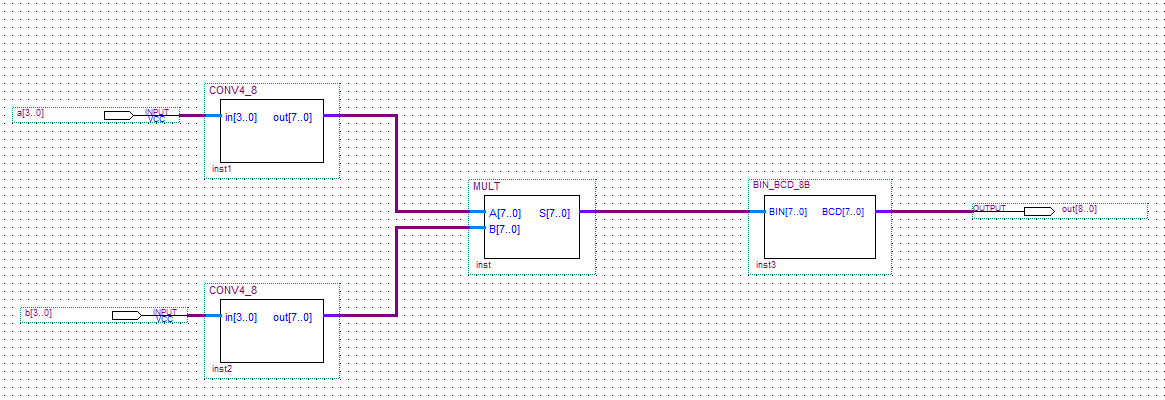
\includegraphics[width=130mm]{Mult_Bin_BCD.jpeg}
		\end{center}
	\end{figure}
	
	\begin{table}[h!]
		\centering
		 \begin{tabular}{|c | c|} 
			 \hline
			 Entrades & Descripció\\ [0.5ex] 
			 \hline
			 a(4) &  Nombre a de 4 bits que es vol multiplicar\\ 
			 b(4) &  Nombre b de 4 bits que es vol multiplicar\\ 
			 \hline\hline
			 Sortides & Descripció\\ [0.5ex] 
			 \hline
			out (8) & Sortida de 8 bits amb el resultat de la multiplicació\\ 
			 \hline
		 \end{tabular}
	\end{table}
	
	FALTA SIMULACIO
	
	Podem veure que funciona a partir de la simulacio ja que retorna la multiplicacio de a i b en BCD ja que representem la solucio en hexadecimal.
	
	\subsection{Bloc sel}
	
	Aquest bloc te l'objectiu de retornar un bus de 7 bits amb el nombre $a$ si la entrada $show$ es 1, i 1111111 si la entrada $show$ es 0;
	\begin{figure}[H]
		\begin{center}
		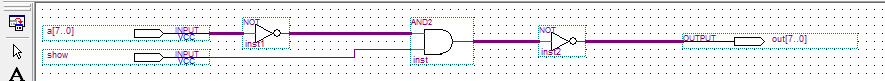
\includegraphics[width=130mm]{SEL.jpeg}
		\end{center}
	\end{figure}
	
	\begin{table}[h!]
		\centering
		 \begin{tabular}{|c | c|} 
			 \hline
			 Entrades & Descripció\\ [0.5ex] 
			 \hline
			 a(8) &  Nombre a seleccionar\\ 
			 show(1) &  Nombre que decideix si la sortida es a o 11111111\\ 
			 \hline\hline
			 Sortides & Descripció\\ [0.5ex] 
			 \hline
			out (8) & Sortida de 8 bits amb el resultat de la multiplicació\\ 
			 \hline
		 \end{tabular}
	\end{table}
	
	\begin{figure}[H]
		\begin{center}
		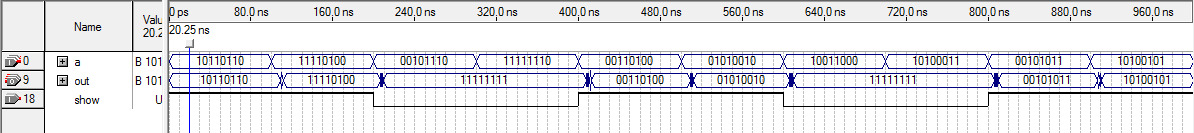
\includegraphics[width=130mm]{Simulacio_Sel.jpeg}
		\end{center}
	\end{figure}
	
	Podem veure que la simulacio funciona ja que si sel es 0 la sortida es 11111111 i si sel es 1 la sortida es a(8).
	
	\subsection{Regs}
	
	Aquest component es un mòdul seqüencial síncron que te com a finalitat carregar i memoritzar els operands de la multiplicació opA i opB. Aquest, si la entrada intro es 1 i clk esta en el flanc de pujada i nrst esta activat, actualitzara els valors de opA i opB, posant a opA el valor entrat per keycode i a opB el antic valor de opA.
	
	\begin{figure}[H]
		\begin{center}
		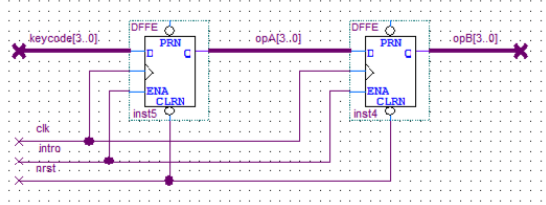
\includegraphics[width=130mm]{regs.png}
		\end{center}
	\end{figure}
	
	\begin{table}[h!]
		\centering
		 \begin{tabular}{|c | c|} 
			 \hline
			 Entrades & Descripció\\ [0.5ex] 
			 \hline
			 keycode(4) & Marca la tecla que s'està prement \\
			 clk(1) & Es el rellotge que gestionara la memoria del sistema\\
			 intro(1) & Indica si s'esta entrant un numero i s'ha d'actualitzar\\
			 nrst(1) & Marcara si s'ha de resetejar a 0 o no \\ [1ex] 
			 \hline\hline
			 Sortides & Descripció\\ [0.5ex] 
			 \hline
			 opA(8) & El valor del nombre A guardat\\
			 opB(8) & El valor del nombre B guardat\\
			 \hline
		 \end{tabular}
	\end{table}
	
	\subsection{control}
	
	Aquest component ens ve donat i esta escrit en vhdl. L'objectiu es guardar el estat en el que estem i indicar als altres moduls si es poden introduir nombres e iluminar els leds verds o mostrar el resultat i iluminar els leds vermells. En el cas que es premi coixinet el estat passarà a ser show, mentres que si es prem asterisc sera intro. Si es prem un nombre el estat es mantindra, i si estem en estat intro, enviara la senyal per a actualitzar els valors de opA i opB. Si estem en estat show no passara res.
	
	
	
	\subsection{Programa principal}
	
	\begin{table}[h!]
		\centering
		 \begin{tabular}{|c | c|} 
			 \hline
			 Entrades & Descripció\\ [0.5ex] 
			 \hline
			 nkey(1) &  Marca si s'esta prement la tecla \\ 
			 keycode(4) & Marca la tecla que s'està prement \\
			 clk(1) & Es el rellotge que gestionara la memoria del sistema  \\
			 nrst(1) & Marcara si s'ha de resetejar a 0 o no \\ [1ex] 
			 \hline\hline
			 Sortides & Descripció\\ [0.5ex] 
			 \hline
			 show(1) & Diu si s'ha de mostrar la sortida o no\\ 
			 opA(8) & El valor del nombre A guardat a regs\\
			 opB(8) & El valor del nombre B guardat a regs\\
			 res(8) & Es el que s'ha de mostrar a la pantalla, la multiplicacio o res\\ [1ex] 
			 \hline
		 \end{tabular}
	\end{table}
	
\end{document}